To write specifications for protocols' rich semantics, I employed ``interaction
tree'' (ITree), a generic data structure for representing interactive programs
in the Coq programming language, introduced by \citet{itree}.  ITree allows
specifying protocols as monadic programs that model valid implementations'
possible behavior.  The model program can be interpreted into a tester program,
to be discussed in later sections.

\subsection{Language definition}
\label{sec:itree-lang}
Consider an echo program, which keeps reading some data and writing it out
verbatim, until reaching EOF:
\begin{coq}
  CoInductive echo := c <- getchar;;
                      if c is EOF then EXIT
                      else putchar c;; echo.
\end{coq}

Here the behavior after \ilc{read} depends on the value actually read.  This
monadic computation can be desugarized into:
\begin{coq}
  CoInductive echo2 := (* equivalent to echo *)
    Bind getchar (fun c => if c is EOF then EXIT
                         else Bind (putchar c) (fun _ => echo)).
\end{coq}

\begin{figure}
\begin{coq}
  CoInductive itreeM (E: Type -> Type) (R: Type) :=
    Ret     : R   -> itreeM E R
  | Trigger : E R -> itreeM E R
  | Bind    : forall {X : Type}, itreeM E X -> (X -> itreeM E R) -> itreeM E R.
\end{coq}
\caption{Mock definition of interaction trees.}
\label{fig:mock-itree}
\end{figure}

\begin{figure}
  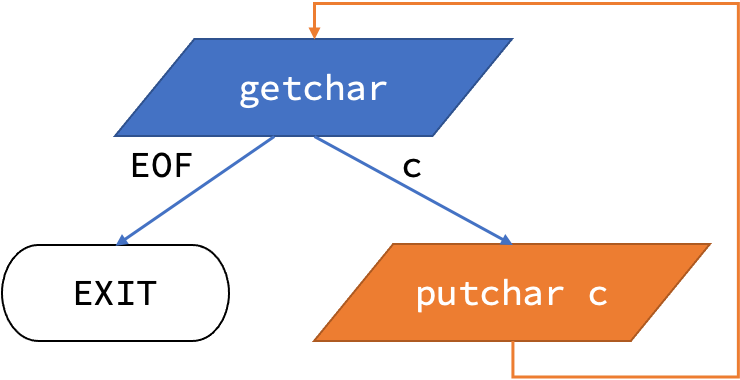
\includegraphics[width=.5\linewidth]{figures/echo-itree}
  \caption{Interaction tree for echo program}
  \label{fig:echo-itree}
\end{figure}

Such continuation-passing style can be represented as a tree of interactions.
To help readers better understand the interaction tree language, I first provide
a modified version of it that better shows its tree structure, and then explain
the actual type definition used in practice.

\paragraph{Mock interaction trees}
As shown in \autoref{fig:mock-itree}, a mock interaction tree (\ilc{itreeM}) has
two kinds of nodes, \ilc{Ret} and \ilc{Trigger}, and has edges constructed by
\ilc{Bind}:
\begin{itemize}
\item \ilc{(Ret r)} represents a pure computation that yields a value \ilc r.
  In the echo example, \ilc{EXIT} halts the program with return value zero:
\begin{coq}
  Definition EXIT {E} : itreeM E Z := Ret 0.
\end{coq}
\item \ilc{(Trigger e)} performs an impure event \ilc e and returns its result.
  Here \ilc{(e: E R)} is an event whose result is of type \ilc R.  For example,
  \ilc{getchar} has result type \ilc{char}, and \ilc{putchar}'s result type is
  \ilc{unit} (which corresponds to \inlinec{void} in C/C++, or \ilc{()} in
  Haskell).  These effective programs are constructed by triggering standard I/O
  events:
\begin{coq}
  Variant stdioE: Type -> Type := (* event type *)
    GetChar:         stdioE char
  | PutChar: char -> stdioE unit.
  
  Definition getchar : itreeM stdioE char := Trigger GetChar.
  Definition putchar (c: char) : itreeM stdioE unit
                               := Trigger (PutChar c).
\end{coq}
\item \ilc{(Bind m k)} binds the return value of \ilc m to the continuation
  function \ilc k.  It first runs program \ilc m until it returns some value of
  type \ilc X.  The return value \ilc{(x: X)} then instantiates \ilc k into the
  following computation \ilc{(k x: itreeM E R)}.  This corresponds to the
  \ilc{(;;)} syntax in \ilc{echo}:
\begin{coq}
  Notation "x <- m1;; m2" := (Bind m1 (fun x => m2)).
  Notation "m1;; m2"      := (Bind m1 (fun _ => m2)).
\end{coq}

As illustrated in \autoref{fig:echo-itree}, each possible return value \ilc x is
an edge that leads to the child it instantiates {\it i.e.} \ilc{(k x)}.  In this
way, the \ilc{Ret} and \ilc{Trigger} nodes are connected into a tree
structure.
\end{itemize}

The mock interaction tree provides an intuitive continuation-passing structure
for representing impure programs.  However, this language is not suitable for
writing specifications and deriving them into tester programs, because the test
derivation requires analyzing and transforming the specification program.

A mock interaction tree has infinitely many syntactic variants that are
semantically equivalent, due to monad laws.  For example, consider the following
programs:
\begin{coq}
  Example bind_ret  r k     := Bind (Ret r) k.
  Example bind_bind m k1 k2 := Bind (Bind m k1) k2.
\end{coq}
These programs are semantically equivalent to:
\begin{coq}
  Example bind_ret2  r k     := k r.
  Example bind_bind2 m k1 k2 := x <- m;; Bind (k1 x) k2.
\end{coq}

To make program analysis more effective, we need to redefine the tree structure
in a normal form, where each semantics corresponds to a unique syntax.  The
revised language eliminates expressions like \ilc{bind_ret} and \ilc{bind_bind}.

\paragraph{Practical interaction trees}
\footnote{For readability, the ``practical'' ITree definition here is a
  simplified version from \citet{itree}.}
\begin{figure}
\begin{coq}
  CoInductive itree (E: Type -> Type) (R: Type) :=
    Pure   : R -> itree E R
  | Impure : forall {X : Type}, E X -> (X -> itree E R) -> itree E R.
\end{coq}
\caption{Formal definition of interaction trees}
\label{fig:itrees}
\end{figure}
The type definition of ITree restricts that only single events can be bound to a
continuation.  As shown in \autoref{fig:itrees}, I use \ilc{(Impure e k)} to
replace \ilc{(Bind (Trigger e) k)} representations in \ilc{itreeM}.  A
\ilc{Pure} computation cannot be bound to a continuation, and must be the leaf
of an ITree.

The \ilc{Ret}, \ilc{Trigger}, and \ilc{Bind} constructors introduced in
\ilc{itreeM} have equivalent representations in \ilc{itree}, so we can still
write programs in the monadic syntax:
\begin{coq}
  Definition ret {E R} : R -> itree E R := Pure.
  
  Definition trigger {E R} (e: E R) : itree E R := Impure e Pure.

  CoFixpoint bind {X E R} (m: itree E X) (f: X -> itree E R) : itree E R :=
    match m with
    | Pure   x   => f x
    | Impure e k => Impure e (fun r => bind (k r) f)
    end.

  Notation "x <- m1;; m2" := (bind m1 (fun x => m2)).
  Notation "m1;; m2"      := (bind m1 (fun _ => m2)).

  CoFixpoint translateM {E R} (m: itreeM E R) : itree E R :=
    match m with
    | Ret     r => ret r
    | Trigger e => trigger e
    | Bind m1 k => x <- translateM m1;; translateM (k x)
    end.
\end{coq}

ITrees can specify various kinds of programs like servers and testers, by
defining different event types.  For example, the QAC server in
\autoref{def:server} exhibits internal nondeterminism.  The internal choices
made by the server can be represented as \ilc{Choice} events whose result can be
any value in the space of choices:
\begin{coq}
  Variant choiceE: Type -> Type :=
    Choice: choiceE C.
\end{coq}

The server also needs to send requests and receive responses:
\begin{coq}
  Variant qaE: Type -> Type :=
    Recv: qaE Q           (* receive a request *)
  | Send: A -> qaE unit.  (* send a response   *)

  Definition qacE: Type -> Type := qaE +' choiceE.
\end{coq}

Here \ilc{qacE} is a sum type of \ilc{qaE} and \ilc{choiceE} events, meaning
that the server may send or receive messages, and may also make internal
choices.  I split the event types because they'll be handled differently when I
derive the tester later in this chapter.

Now we can represent the QAC server with step function \ilc{sstep} and initial
state \ilc{sigma}:
\begin{coq}
  CoInductive server (sstep: Q -> C -> sigma -> A * sigma) (s: sigma)
              : itree qacE void :=
    c <- trigger Choice;;
    q <- trigger Recv;;
    let (a, s') := sstep q c s in
    trigger (Send a);;
    server sstep s'.
\end{coq}

This subsection has provided a brief taste of the ITree specification language.
To construct a tester from the specification, we need to dualize the model's
behavior into the tester-side behavior, based on the theory explained in
\autoref{sec:dualization}.  To dualize specifications written in ITrees, we need
an {\em interpretation} mechanism that transforms ITrees into other programs,
which will be explained in the next subsection.

\subsection{Interpreting interaction trees}
To interpret a program \ilc p is to specify a rule that defines ``if \ilc p does
this, then do that''.  For example, shell syntax \inlinec{(p < input > output)}
executes \inlinec p but redirects its standard I/O.  Suppose \inlinec p is the
\ilc{echo} program in \autoref{sec:itree-lang}, then the redirected program
should perform file operations specified in \ilc{redirect_echo}:
\begin{coq}
  Variant fileE: Type -> Type :=      (* file operation events *)
    Fgetc: file ->         fileE char
  | Fputc: file -> char -> fileE unit.

  CoInductive redirect_echo (input output: file) : itree fileE unit :=
    c <- trigger (Fgetc input);;
    if c is EOF then ret 0
    else trigger (Fputc output c);;
         redirect_echo input output.
\end{coq}

When redirecting a program's standard I/O to files, the interpretation rule is
``whenever the program wants to read from or write to standard I/O, perform the
read/write operation on the specified file instead'':
\begin{coq}
  Definition redirect (input output: file) {R: Type} (e: stdioE R) :=
    match e in stdioE R return itree fileE R with
    | GetChar   => trigger (Fgetc input)
    | PutChar c => trigger (Fputc output c)
    end.
\end{coq}

Here the \ilc{redirect} function takes a standard I/O event and turns it into an
ITree program that performs file events.  The result program has the same return
type as the original event, so it can ``replace'' the original \ilc{stdioE}.
This is done by the \ilc{interp} function:
\begin{coq}
  CoFixpoint interp {E F R} (f: forall {T}, E T -> itree F T) (m: itree E R)
             : itree F R :=
    match m with
    | Pure   r   => Pure r
    | Impure e k => x <- f e;;
                    interp handler (k x)
    end.

  Definition redirect_echo2 (input output: file) : itree fileE unit :=
    interp (redirect input output) (translateM echo).
\end{coq}

For each impure event, the interpretor replaces it with the program defined by
the handler function \ilc f.  As a result, \ilc{redirect_echo2} constructs a
redirected echo program that is equivalent with \ilc{redirect_echo}.

To derive tester programs from ITree specifications, I'll introduce multiple
interpretation processes, with various event handlers throughout this chapter.
